\documentclass[a4paper,11pt,twoside]{article}
%\documentclass[a4paper,11pt,twoside,se]{article}

\usepackage{UmUStudentReport}
\usepackage{verbatim}   % Multi-line comments using \begin{comment}
\usepackage{courier}    % Nicer fonts are used. (not necessary)
\usepackage{pslatex}    % Also nicer fonts. (not necessary)
\usepackage[pdftex]{graphicx}   % allows including pdf figures
\usepackage{listings}
\usepackage{pgf-umlcd}
%\usepackage{lmodern}   % Optional fonts. (not necessary)
%\usepackage{tabularx}
%\usepackage{microtype} % Provides some typographic improvements over default settings
%\usepackage{placeins}  % For aligning images with \FloatBarrier
%\usepackage{booktabs}  % For nice-looking tables
%\usepackage{titlesec}  % More granular control of sections.

% DOCUMENT INFO
% =============
\department{Department of Computing Science}
\coursename{Object-Oriented Programming Methodology 7.5 p}
\coursecode{5DV133}
\title{OU2 Robots and Labyrinths}
\author{Lorenz Gerber ({\tt{dv15lgr@cs.umu.se}} {\tt{lozger03@student.umu.se}})}
\date{2016-04-25}
%\revisiondate{2016-01-18}
\instructor{Anders Broberg / Niklas Fries / Adam Dahlgren / Jonathan
  Westin / Erik Moström / Alexander Sutherland}


% DOCUMENT SETTINGS
% =================
\bibliographystyle{plain}
%\bibliographystyle{ieee}
\pagestyle{fancy}
\raggedbottom
\setcounter{secnumdepth}{2}
\setcounter{tocdepth}{2}
%\graphicspath{{images/}}   %Path for images

\usepackage{float}
\floatstyle{ruled}
\newfloat{listing}{thp}{lop}
\floatname{listing}{Listing}



% DEFINES
% =======
%\newcommand{\mycommand}{<latex code>}

% DOCUMENT
% ========
\begin{document}
\lstset{language=C}
\maketitle
\thispagestyle{empty}
\newpage
\tableofcontents
\thispagestyle{empty}
\newpage

\clearpage
\pagenumbering{arabic}

\section{Problem Description} 
Aim of this laboration was to implement a number of class that allow
to simulate robots in a labyrinth. The assignment suggested three base
classes \textit{Maze}, \textit{Position} and \textit{Robot}
\cite{maze}. Further, it was defined that two specializations of the
\textit{Robot} class had to be implemented: One robot that always
follows with his `right hand' along the wall until he finds the
goal of the maze. And another one that can remember positions where he has
been and hence look for new unexplored positions until he finds the exit.

The classes were to be tested in a \textit{main} program. More
specific, the two specialized robot classes should be evaluated in a
competition against each other. The maze shall be provided as text
file in the command line arguments. 

\section{Usage Instructions}


\section{System Description}
\subsection{UML class diagram}
\begin{figure}
\centering
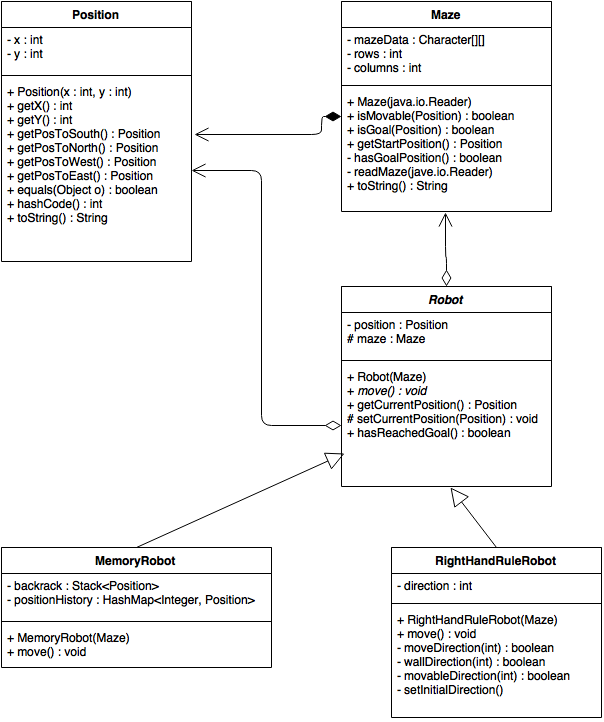
\includegraphics[width=\textwidth]{maze.png}
\caption{This is the UML class diagram}
\label{fig:UML}
\end{figure}

\subsection{Class Responsibilty and Collaborations}
\subsection{Specific Implementation details}

\subsection{Move Algorithms of the Robots}
\subsubsection{Right Hand Rule Robot}
The right hand rule robot needed a number of help methods besides the
specified \textit{move()} method. This was mainly a consequence for
giving the robot a memory for the direction of movement. This was seen
as a measure to model the behaviour of the robot as close as possible
how a physical implementation would work: If a robot has a
\textit{right hand}, it also has a direction and all operations should
relate to the direction of the robot. The private methods
\textit{moveDirection()}, \textit{wallDirection} and
\textit{movableDirection} are used to lookup geographic directions
from robot directions. The actual translation is done in the
\textit{move()} method using addition and subtraction followed by a
modulo operator on a direction value that is initialized by the
\textit{setInitialDirection()} method.

\textit{Try...catch} statements are used to handle
\textit{ArrayIndexOutOfBounds} exceptions when the robot is at the
edge of the maze. The edge is interpreted as a wall. 

\subsubsection{Memory Robot}
The memory robot needs just the specified \textit{move()} method. It
uses a \textit{stack} (\textit{java.util.Stack}) for
implementing the back tracking and a hash table
(\textit{java.util.HashMap}) for the memory of already visited
places. For this work, the \textit{hashCode()} method of the
\textit{Position} Class had to be implemented with an override. It was
chosen to concatenate the X and Y position with an arbitrary
unlikely-to-appear number (`9999' was chosen here).  

The \textit{move()} method of the memory robot can be roughly
separated in two parts. In the first part, the robot checks in every
four directions the possibility to move based on the condition
\textit{isMovable} from the \textit{Position} class and whether the
\textit{hashCode} of the potential new position is already stored in
the \textit{positionHistory} hash map. In the current version, a fixed
sequence of direction is implemented (North, East, South, West). As
soon as a viable directin is found, the robot makes the move. This
includes pushing the current position on the \textit{backtrack} stack,
storing the hash code of the current position to the
\textit{positionHistory} hash map and finally, changing location to
the new position. After making the move, the method is left with a
return statement without reaching the second part. Each of the
direction checking code blocks is enclosed in a \textit{try...catch}
statement that handles the \textit{ArrayIndexOutOfBounds} exception
when the robot is at the edge of the maze. Hence positions `beyond'
the maze are interpreted as wall.


The second part of the \textit{move()} method in the memory robot is
concerned with the backtracking. It consists just of reading the stack
for the last position, and then popping the top of the stack. As
mentioned above, this second part is just reached when no direction
offered a viable move. 



\section{Known Limits}
The robots are implemented such that they accept the border of the
maze as a wall. Hence a valid maze without any wall can be created.

In the current version, the \textit{Memory Robot} will not detect when
there is no solution to the maze. This could be implemented by
checking for the start position after back tracking.

\section{Testing}
\subsection{JUnit tests}
As requested, JUnit tests were implemented for the classes
\textit{Maze} and \textit{Position}. The test were implemented post
development of the main code.

\subsubsection{Maze}
The JUnit test for maze verify whether a correct Maze can be
loaded. Then each a test to check for exceptions when a maze without
start or goal position, or a maze with uneven row length is attempted
to load. 

\subsubsection{Position}
JUnit tests to check whether a \textit{Position} object can be
instantiated and to verify that the \textit{equals()} method works
were implemented. Further, it is checked whether different positions
yield different hash codes. 

\subsection{Run tests and Robot tests}
The robot testing was implemented in a small main program. A static
variable \textit{ROUNDS} determine how many rounds the competition
shall last. This mode was decided as it would be more difficult to
detect adhoc whether a maze can be 'solved' in general or by a
specific robot particularly. So, limiting to a fixed number of rounds
was a mean to prevent infinite looping. A typical situation where
an infinite loop could occur is when a robot starts within a
compartment that has no connection to the compartment with the
\textit{Goal} position.

Move counters for each robot are used. In each round, it is first
checked whether either of the robots has reached the
\textit{Goal}. Then the move counter is advanced by one and the the
\textit{move()} method of each robot is called.  After the predefined
number of rounds are over, it is evaluate whether the robots reached
the goal and if so, which one reached it first.

For testing purposes, \textit{toString()} methods for
\textit{Position} and \textit{Maze} were implemented. They were used
during development to verify the correctness of the algorithms. 

The text files \textit{maze1.txt} and \textit{maze2.txt} work with
both robots, while \textit{maze3.txt} results in an exception for the
right hand rule robot as the starting position is not at a wall. The
other provided maze text files are used for the JUnit testing and
produce exceptions. 

\addcontentsline{toc}{section}{\refname}
\bibliography{references}

\end{document}
